% 中文单栏技术报告模板：真实数学排版、三线表、可点击目录与矢量插图。
% 借鉴学术单栏稿件的结构，不宣称采用训练营或 ACM 官方出版模板。
\documentclass[UTF8,a4paper,zihao=5,fontset=none]{ctexart}
\setCJKmainfont[BoldFont=STHeitiSC-Medium]{Songti SC}
\setCJKsansfont{Heiti SC}
\setCJKmonofont{Heiti SC}
\usepackage[left=24mm,right=24mm,top=23mm,bottom=23mm,headheight=15pt]{geometry}
\usepackage{amsmath,amssymb,bm}
\usepackage{graphicx,booktabs,array,longtable,float}
\usepackage{fancyhdr,fvextra,xcolor,caption,needspace}
\usepackage[unicode,hidelinks,bookmarksnumbered]{hyperref}
\setmainfont{Times New Roman}
\setsansfont{Helvetica Neue}
\setmonofont[Scale=0.90]{Menlo}
\linespread{1.12}
\setlength{\parindent}{2em}
\setlength{\parskip}{2pt}
\setlength{\emergencystretch}{2em}
\clubpenalty=10000
\widowpenalty=10000
\displaywidowpenalty=10000
\renewcommand{\topfraction}{0.88}
\renewcommand{\bottomfraction}{0.85}
\renewcommand{\textfraction}{0.10}
\renewcommand{\floatpagefraction}{0.72}
\makeatletter
\setlength{\@fptop}{0pt}
\setlength{\@fpsep}{16pt}
\makeatother
\ctexset{section={format=\large\bfseries,beforeskip=16pt,afterskip=8pt},
  subsection={format=\normalsize\bfseries,beforeskip=11pt,afterskip=5pt},
  subsubsection={format=\normalsize\bfseries,beforeskip=8pt,afterskip=4pt}}
\captionsetup{font=small,labelfont=bf,labelsep=quad,skip=6pt}
\renewcommand{\tablename}{表}
\renewcommand{\figurename}{图}
\renewcommand{\refname}{参考文献}
\setlength{\LTpre}{6pt}
\setlength{\LTpost}{8pt}
\setlength{\tabcolsep}{4pt}
\renewcommand{\arraystretch}{1.18}
\newcolumntype{P}[1]{>{\raggedright\arraybackslash}p{#1}}
\newcolumntype{C}[1]{>{\centering\arraybackslash}p{#1}}
\newcolumntype{R}[1]{>{\raggedleft\arraybackslash}p{#1}}
\DefineVerbatimEnvironment{ReportCode}{Verbatim}{fontsize=\small,
  breaklines=true,breakanywhere=true,frame=single,rulecolor=\color{black!25},
  framesep=5pt,baselinestretch=1.04}
\pagestyle{fancy}
\fancyhf{}
\fancyhead[L]{\small 任务 9\quad 技术报告}
\fancyhead[R]{\small GPU 向量检索引擎}
\fancyfoot[C]{\small\thepage}
\renewcommand{\headrulewidth}{0.35pt}
\hypersetup{pdftitle={百万级 GPU 向量检索引擎的设计、验证与性能分析},pdfsubject={2026夏季训练营 CUDA 方向技术报告},
  pdfcreator={Tectonic / XeLaTeX},pdfauthor={}}
\begin{document}
\thispagestyle{empty}
\begin{center}
{\small 2026 夏季训练营 CUDA 方向项目\quad 任务 9}\par
\vspace{11pt}
{\LARGE\bfseries 百万级 GPU 向量检索引擎的设计、验证与性能分析\par}
\vspace{8pt}
{\normalsize Design and Evaluation of a GPU Vector Retrieval Engine\par}
\end{center}
\vspace{4pt}
\noindent\textbf{摘\quad 要}\quad 本报告设计并实现了包含精确检索与 IVF-Flat 索引的 CUDA 向量检索引擎，研究距离计算、候选生成和 Top-K 选择对完整查询性能的影响。系统支持 L2 平方距离、内积和余弦相似度，FP32/FP16 文件输入，以及 $K\in\{1,10,50,100\}$。30 个 CPU/GPU 正确性用例全部通过，同一向量 ID 的最大分数绝对误差为$1.53\times10^{-5}$。在 RTX 5090 上，对 1,000,000 条 128 维向量执行 1,000 条查询时，精确检索在 $K=10$ 下达到 $1488.2\pm3.2$ QPS，逐查询 P99 计时的重复均值为 0.530 ms；前 20 条相同查询相对于单线程 CPU 参考实现的热路径加速比为 $144.7\times$。IVF 索引构建耗时 1.596 s，在 $\mathrm{nprobe}=1$时对 20 条质量查询取得 $\mathrm{Recall@10}=1$，吞吐为 $1327.6\pm3.1$ QPS，低于 GPU 精确检索。Nsight Systems 显示，精确检索的评分内核占设备内核时间的 89.5\%，IVF 的完整排序占 67.1\%。实验说明，候选数缩减带来的计算收益需要与主机粗检索、候选处理和排序成本共同评估。本文据此提出针对两条检索路径的优化顺序，并说明合成数据、质量样本量及计时边界对结论的影响。上述 $\pm$表示重复运行的样本标准差。\par
\vspace{5pt}
\noindent\textbf{关键词}\quad  向量检索；CUDA；Top-K；IVF-Flat；近似最近邻；尾延迟\par
\vspace{6pt}
\section{引言}

检索增强生成、推荐和多模态系统需要从大规模高维向量库中返回有序 Top-K。GPU 适合并行距离计算，但检索系统的吞吐还受候选生成、选择算法、数据传输和批处理调度影响。已有 GPU 相似性检索工作表明，选择算法与内存层次的设计是发挥设备并行能力的重要组成部分 \cite{r1}。对近似检索而言，性能还需与召回率共同评估，才能反映索引引入的实际取舍。


现有向量检索系统主要在访问范围、向量表示和设备执行方式之间进行取舍。Faiss 将精确扫描、倒排索引、向量压缩和图索引组织为可组合的检索组件，强调精度、查询成本、存储与构建成本之间的联系 \cite{r2}。其中，IVF 根据粗量化中心缩小访问范围；乘积量化（PQ）将向量分解到多个子空间并以短码近似表示，进一步降低存储和距离计算成本 \cite{r3}；HNSW 则通过分层邻接图导航候选 \cite{r4}。三者分别改变候选访问或数据表示，不宜仅依据某一次吞吐数字判断其适用性。


本文选取保留原始向量的 IVF-Flat，使近似误差主要来自候选筛选，而非额外的PQ 重构误差。精确扫描与 IVF 候选重排共用评分和排序内核，因而能够在同一计算语义下观察候选缩减的效果。该选择有利于拆解系统成本，但并不覆盖向量检索的完整设计空间：PQ 与 HNSW 在本文中仅作为方法背景，未进入实测对照。


评估方法同样影响算法比较。ANN-Benchmarks 通过统一接口、数据集与参数扫描比较质量和查询效率，说明召回率应与性能共同报告 \cite{r5}。本文沿用这种联合观察的思路，但实验由自建驱动执行，输入为可控合成数据。对于 GPU Top-K，Johnson 等研究了面向寄存器和线程束的选择算法 \cite{r1}，RadiK 则研究基于基数划分的选择及其随输入长度、$K$ 和批大小变化的行为 \cite{r6}。这些工作表明，完整排序并非获取 Top-K 的唯一方式，也为本文的内核成本分析提供了参照。


本文采用独立的 CPU 堆选择算法与 CUDA 基数排序建立精确检索基线，并在此基础上加入可持久化的 IVF-Flat 索引。实现覆盖二进制输入、索引构建与加载、批量查询、结果输出以及质量和性能日志，实验则将小规模数值验证与百万级性能评估分开开展。本文的贡献是可复查的系统实现与实验分析，而非新的近邻索引或Top-K 算法。重点考察既有算法在当前 CPU/GPU 分工下的行为，并以观测到的成本结构提出可验证的改进方向。


实验围绕三个问题展开：精确检索的开销如何随 $K$ 变化；IVF 的候选缩减能否转化为完整查询加速；探测桶数和查询批大小如何影响召回率、吞吐及尾部计时。第 3-4 节介绍算法与系统，第 5-7 节说明实验方法并分析结果，第 8-10 节讨论数值验证与实现取舍、有效性及后续优化。


\section{问题定义与实验配置}

\par\medskip\noindent\begin{minipage}{\linewidth}
\small
\captionof{table}{正式实验环境与数据规模}\label{tab:1}
\begin{tabular}{@{}P{41.389mm}P{117.799mm}@{}}
\toprule
\textbf{项目} & \textbf{正式实验配置} \\
\midrule
GPU & NVIDIA GeForce RTX 5090，32,607 MiB，计算能力 12.0 \\
驱动 / CUDA & NVIDIA driver 610.43.02；CUDA Toolkit 12.8.61 \\
编译环境 & CMake 3.31.4；G++ 13.3.0；Release + {\small\ttfamily -\allowbreak{}lineinfo} \\
数据规模 & $N=1{,}000{,}000$，$D=128$，$Q=1{,}000$ \\
IVF & $\mathrm{nlist}=4096$；训练样本 65,536；Lloyd 迭代 2 次 \\
质量评估 & 20 条查询，CPU 精确检索作为真值 \\
随机数设置 & 固定主种子，随数据元信息记录 \\
重复 & 精确检索 3 次；IVF 5 次；每组预热 1 次 \\
\bottomrule
\end{tabular}
\end{minipage}\par\medskip

表 1 列出正式实验配置。性能测试采用 FP32 输入与 L2 平方距离。数据由 4096 个标准正态中心生成，每条库向量叠加标准差 0.15 的高斯噪声；查询从库向量抽样后叠加标准差 0.02 的噪声。这一设计使查询与库高度相关，便于控制规模和验证检索链路。索引训练从数据库按种子偏移进行等距采样。数据生成使用 NumPy 1.26.4。数据库与查询文件分别为512,000,028 和 512,028 字节。


\section{检索算法与数据布局}

\subsection{精确检索}

设数据库为 $X=\{\boldsymbol{x}_i\}_{i=1}^{N}$，其中$\boldsymbol{x}_i\in\mathbb{R}^{D}$，查询向量为 $\boldsymbol{q}$。三种评分函数定义为


\nopagebreak[4]
\begin{equation}
\label{eq:1}
\begin{aligned}
s_{\mathrm{L2}}(\boldsymbol{q},\boldsymbol{x})
  &= \sum_{d=1}^{D}(q_d-x_d)^2,\\
s_{\mathrm{IP}}(\boldsymbol{q},\boldsymbol{x})
  &= \sum_{d=1}^{D}q_dx_d,\\
s_{\mathrm{cos}}(\boldsymbol{q},\boldsymbol{x})
  &= \frac{\sum_{d=1}^{D}q_dx_d}
  {\lVert\boldsymbol{q}\rVert_2\lVert\boldsymbol{x}\rVert_2}.
\end{aligned}
\end{equation}

L2 按升序返回结果，内积和余弦相似度按降序返回；省略 L2 的平方根不改变Top-K 次序。任一向量范数为零时，余弦相似度定义为零。CPU 与 CUDA 均使用FP32 累加，严格同分时优先返回较小 ID。


GPU 每个线程块包含 256 个线程，通过网格步长循环分配候选。每个线程顺序遍历一条向量的 $D$ 个分量，将评分与 ID 写入两个数组，再由 CUB DeviceRadixSort完成全量排序 \cite{r7}。精确检索的输入 ID 按自然顺序排列；IVF 在主机端先将候选ID 排序，两条路径均利用稳定排序实现同分 ID 规则。


单查询评分的工作量为 $O(ND)$；32 位排序键对应固定轮数的基数排序，其工作量和临时空间均随 $N$ 线性增长。CPU 参考实现使用容量为 $K$ 的堆，时间上界为$O(ND+N\log K)$，附加堆空间为 $O(K)$。两者采用不同的选择算法，便于独立核对结果。全排序 CUDA 基线在 $K=1$ 时也处理全部 $N$ 个分数，这构成后续采用专用 Top-K 选择算法的优化空间。


\subsection{IVF-Flat}

索引包含 $L=\mathrm{nlist}$ 个聚类中心。训练阶段对 $S$ 个样本执行 $I$ 次Lloyd 迭代 \cite{r8}，CUDA 负责分配，CPU 以 FP64 求和更新中心。以下以$\boldsymbol{x}_i$ 表示采样后的训练向量，L2 模式的迭代写为


\nopagebreak[4]
\begin{equation}
\label{eq:2}
\begin{aligned}
a_i^{(t)} &= \arg\min_{1\le j\le L}
  \lVert\boldsymbol{x}_i-\boldsymbol{c}_j^{(t)}\rVert_2^2,\\
\mathcal{C}_j^{(t)} &= \{i:a_i^{(t)}=j\},\\
\boldsymbol{c}_j^{(t+1)} &=
  \frac{1}{\lvert\mathcal{C}_j^{(t)}\rvert}
  \sum_{i\in\mathcal{C}_j^{(t)}}\boldsymbol{x}_i,
  \qquad \lvert\mathcal{C}_j^{(t)}\rvert>0.
\end{aligned}
\end{equation}

空簇用确定性样本重置。余弦模式在均值更新后归一化中心；内积模式使用最大内积分配和均值更新。训练完成后，CUDA 对全库执行一次分配，CPU 构造 CSR形式的 {\small\ttfamily offsets[L+1]} 与 {\small\ttfamily ids[N]}。分配阶段的主要工作量为$O(ISLD+NLD)$，中心更新为 $O(ISD)$。


查询首先在 CPU 上计算并排序 $L$ 个中心评分，选择前 {\small\ttfamily nprobe} 个倒排表，合并候选 ID 并按 ID 排序。若候选不足 $K$，则继续访问后续倒排表，直至候选充足或遍历全部倒排表。GPU 随后读取 $C$ 个候选的原始向量，计算评分并排序。单查询主机工作量为 $O(LD+L\log L+C\log C)$，设备评分工作量为 $O(CD)$，设备端仍采用全量基数排序。IVF-Flat 保留未压缩向量；它通过缩减 $C$ 降低评分成本，同时引入粗检索和候选处理开销，二者共同决定最终性能。


在倒排表长度相近的理想情形下，候选数可粗略写作$C\approx N\,\mathrm{nprobe}/L$；实际值还取决于簇不均衡、查询分布及候选不足时的追加探测 \cite{r2}。因此本文报告真实候选数，而不以该近似替代测量。正式索引只执行两次聚类迭代，这一设置固定了构建预算；其结果用于当前索引的性能分析，不能视为对聚类收敛或最优探测参数的证明。


\subsection{精度、数据布局与批处理}

数据库与查询均按行主序存储。FP16 文件读入后解码为 FP32，后续评分与索引计算使用 FP32。当前“一线程一向量”的映射便于统一三种度量，但同一线程束在相同维度读取相邻向量时，地址间隔为 $D$ 个 float；在 $D=128$ 时，改用线程束协同处理一条向量或分块布局，可能改善访存效率。这一判断来自地址布局与 CUDA 合并访存原则 \cite{r9}；实际收益还受缓存复用、归约指令和寄存器需求影响，需要通过实现对照而非仅凭步长推断。


{\small\ttfamily batch\_\allowbreak{}size} 定义查询循环的分组边界，一次调用可处理 $Q$ 条查询。组内各查询依次完成主机到设备传输（H2D）、评分、排序和设备到主机传输（D2H），当前执行方式为串行调度。第 6.4 节以批大小扫描检验这一接口在现有实现中的作用。


\section{系统实现}

\subsection{索引持久化与接口职责}

二进制数据库和查询文件使用小端序，文件头包含格式标识、版本、int64 数量、int32 维度和数据类型/度量枚举，具体编码见 README。索引使用 {\small\ttfamily IVFFLT1}标识和版本 1；32 字节文件头后依次存放 FP32 {\small\ttfamily centers[L\ensuremath{\times}D]}、uint64 {\small\ttfamily offsets[L+1]} 与 int64 {\small\ttfamily ids[N]}。原始向量保存在独立数据库文件中，查询时同时加载数据库和索引。读取过程检查维度、版本、偏移单调性、ID 范围及文件长度，实验清单还记录文件哈希以固定输入。


数据库、评分数组、ID 数组及 CUB 工作区在一次查询调用内分配并复用，$Q=1000$ 的查询序列仅上传一次数据库，调用结束后释放设备缓冲区。IVF 的中心、倒排偏移和 ID 保存在主机端：CPU 先生成全部查询的候选列表，GPU 再逐查询接收候选 ID 并执行评分与排序。该设计降低了重复分配和数据库传输成本，也使主机候选处理成为值得单独分析的阶段。


主程序分别写出检索结果、质量日志与性能日志。CUDA 后端与 CPU 参考实现共用输入解析及索引接口；无 CUDA 环境使用替代链接模块，仍可执行文件解析、CPU检索和索引保存/加载测试。


持久化索引描述中心与倒排关系，向量值由独立数据库提供。因而“索引文件大小”与检索所需的总存储不同：前者不包含原始向量，后者还应计入数据库及运行时工作区。构建、加载、查询和质量评价采用分离接口，使索引构建时间不必在每次搜索中重复支付，也便于区分数值参考计算与待测查询路径。


\subsection{工作区规模与候选访问}

设单次调用中的最大候选数为 $C_{\max}$，CUB 临时工作区为$W_{\mathrm{CUB}}$ 字节。根据 FP32 分数与 int64 ID 的显式分配，设备工作集为


\nopagebreak[4]
\begin{equation}
\label{eq:3}
M_{\mathrm{dev}}=4ND+4D+24C_{\max}
 +8C_{\max}\mathbf{1}_{\mathrm{IVF}}+W_{\mathrm{CUB}}.
\end{equation}

其中 $24C_{\max}$ 包含分数与 ID 的输入/输出双缓冲；IVF 另需候选 ID 数组。精确检索取 $C_{\max}=N$。这解释了候选缩减主要减少临时工作区，而数据库常驻部分保持不变。CPU 保存全部查询候选还需要$O(\sum_{q=1}^{Q}C_q)$ 的 ID 空间，该部分不在设备工作集指标内。


CSR 使每个倒排表的 ID 连续，但向量值仍按原始数据库顺序排列，候选评分需要间接寻址。将 ID 排序保证了稳定的同分规则，并不等价于将每个簇的向量重排为连续设备存储。后续若按倒排表物理重排向量，需要同时维护原始 ID 映射，并把重排成本计入构建时间；否则查询加速与额外预处理之间的取舍将不完整。


\section{实验方法}

\subsection{验证方案与质量指标}

正确性矩阵使用 $N=4096$、$D=64$、$Q=32$ 和 32 个合成簇。精确检索覆盖三种度量、两种文件精度和四个 $K$；IVF 使用 $K=10$、$\mathrm{nlist}=32$、$\mathrm{nprobe}=8$，共计 30 个用例。验证种子由固定主种子与度量、精度对应的偏移确定，并随配置保存。IVF 的 CPU/CUDA 路径加载同一份 GPU 构建索引，以检验搜索结果的一致性。


设质量查询数为 $Q_g$，预测与真值的 Top-K 集合分别为 $\mathcal{A}_q$ 和$\mathcal{T}_q$，第 $k$ 个返回位置的分数分别为 $\widehat{s}_{qk}$ 与$s_{qk}^{\star}$。质量日志使用


\nopagebreak[4]
\begin{equation}
\label{eq:4}
\begin{aligned}
\mathrm{Recall@K}
  &=\frac{1}{Q_gK}\sum_{q=1}^{Q_g}
    \lvert\mathcal{A}_q\cap\mathcal{T}_q\rvert,\\
E_{\mathrm{rank}}
  &=\frac{1}{Q_gK}\sum_{q=1}^{Q_g}\sum_{k=1}^{K}
    \lvert\widehat{s}_{qk}-s_{qk}^{\star}\rvert.
\end{aligned}
\end{equation}

其中 $E_{\mathrm{rank}}$ 为平均位置分数误差，同时反映返回邻居差异和浮点舍入。验证脚本还按同一 ID 对齐评分，计算平均及最大绝对误差，并分别保留严格排序一致率与容差排序一致率。


这些指标回答不同问题。集合召回率度量是否找到参考邻居，但不描述顺序；同 ID 分数误差隔离评分计算差异；位置分数误差则同时受邻居替换影响。本文将三者结合，以避免平均分数相近掩盖漏检。这里的“精确检索”指穷举全库，其评分仍遵循 FP32 浮点运算，并非无限精度的数学真值。IVF 验证中固定索引，首先隔离搜索后端的一致性；独立训练索引的质量属于另一项实验问题。


正式实验使用第 2 节的百万级数据：精确检索重复 3 次，IVF 重复 5 次，每组先进行一次不计入汇总的完整预热。每次重复启动独立进程，显存和 CUDA 上下文不会跨进程复用。吞吐使用全部 1000 条查询，质量指标和 CPU 参考计时使用固定前 20 条查询。各次重复共享数据与索引，标准差用于刻画运行时间波动。同一查询返回的 $K$ 个邻居并非独立样本，不能把 $20K$ 个命中项直接当作独立伯努利试验来估计总体召回置信区间。本文仅报告这组查询的经验召回率，并将更大、独立查询集上的质量-性能曲线作为后续评估目标 \cite{r5}。


\subsection{性能指标与计时边界}

设完整查询耗时为 $T_{\mathrm{query}}$（ms），吞吐定义为


\nopagebreak[4]
\begin{equation}
\label{eq:5}
\mathrm{QPS}=\frac{1000Q}{T_{\mathrm{query}}}.
\end{equation}

计时在数据库和查询文件读取后开始，覆盖查询调用内的显存分配与释放、一次数据库上传以及全部查询；IVF 还包括索引加载、CPU 中心排序和候选拼接。结果写出及随后执行的 CPU 真值计算位于计时区间之外。


单查询计时包含查询与候选 H2D、评分、排序、结果 D2H 及同步；IVF 加上该查询在前置阶段测得的粗检索与候选处理时间。它排除一次性显存分配、数据库上传和索引加载。由于 CPU 先处理全部粗检索，再开始 GPU 阶段，IVF 计时是分段工作时间之和，与在线请求从到达到返回的响应延迟有所区别。


每次重复内对 1000 个单查询时间升序排列为 $t_{(1)},\ldots,t_{(Q)}$，分位数采用 nearest-rank 定义：


\nopagebreak[4]
\begin{equation}
\label{eq:6}
P_p=t_{(\lceil pQ\rceil)},\qquad p\in\{0.50,0.99\}.
\end{equation}

表中 P50/P99 为各次重复分位数的平均值；QPS 标准差采用样本标准差，即分母为重复次数减一。CPU 加速比使用同次运行的前 $Q_g=20$ 条查询，定义为


\nopagebreak[4]
\begin{equation}
\label{eq:7}
S_{\mathrm{CPU/GPU}}=
\frac{\sum_{q=1}^{Q_g}t_q^{\mathrm{CPU}}}
     {\sum_{q=1}^{Q_g}t_q^{\mathrm{GPU}}}.
\end{equation}

最终加速比为各次重复比值的均值。CPU 采用单线程 C++ 堆参考实现；该比值对应相同查询的热路径，因此与全量 QPS 除以采样 CPU QPS 的结果不同。


显存指标统计查询期间显式分配的数据库、查询、评分/ID 双缓冲、IVF 候选 ID和 CUB 工作区，作为设备工作集估算。建索引时间则覆盖采样、聚类迭代、全库分配、倒排表生成与索引落盘，数据库文件读取不计入其中。


\subsection{重复设计与比较原则}

性能统计的观测单元是一次完整进程运行，而非将进程内的 1000 条查询当作1000 次独立系统实验。精确检索的三次重复和 IVF 的五次重复分别形成均值及样本标准差；P99 是各次运行内的尾部分位数，不能与运行间标准差互换。一次预热可减轻首次执行影响，但后续独立进程仍会重新创建设备资源。因此，本文的完整调用结果包含初始化成本，热路径计时则描述另一种使用边界。


参数扫描保持数据、评分精度和真值查询集合不变，分别改变 $K$、探测桶数或分组大小。跨算法比较同时给出召回率、候选数与完整调用性能，不把减少候选视为加速的充分条件。若将来加入 Faiss 或 HNSW 对照，应对齐输入精度、质量目标、线程数、设备驻留方式和结果传输范围，而不能直接引用其论文中的速度与本实验相除。当前单线程 CPU 实现承担独立参考职责，不代表经过优化的CPU 检索系统所能达到的性能上限。


\section{实验结果}

\subsection{正确性与索引构建}

表 2 汇总 30 个验证用例，全部通过。最低严格排序一致率为 0.998750，容差排序一致率为 1，说明差异集中于近同分候选的位置交换。


\par\medskip\noindent\begin{minipage}{\linewidth}
\small
\captionof{table}{CPU/CUDA 正确性验证汇总}\label{tab:2}
\begin{tabular}{@{}P{101.881mm}R{57.308mm}@{}}
\toprule
\textbf{检查项} & \textbf{结果} \\
\midrule
通过用例 & 30/30 \\
最低 Top-K 集合召回率 & 1.000000 \\
最低严格排序一致率 & 0.998750 \\
最低容差排序一致率 & 1.000000 \\
各用例同 ID 平均分数绝对误差的最大值 & $1.829125\times10^{-6}$ \\
全矩阵同 ID 最大分数绝对误差 & $1.53\times10^{-5}$ \\
\bottomrule
\end{tabular}
\end{minipage}\par\medskip

例如，L2/FP16、$K=100$ 的严格排序一致率为 0.999375，余弦/FP32、$K=100$为 0.998750，两者返回 ID 集合均完全一致。验证使用预设绝对容差$\tau=2\times10^{-4}$：逐位置 ID 相同则判为一致；ID 不同时，要求整条查询的 ID 集合相同且对应位置的分数差不超过 $\tau$。全用例同时要求同 ID 最大分数误差不超过 $\tau$，由此区分浮点近同分换位与邻居漏检。


百万级 IVF 索引单次构建耗时为 1596.375828 ms，索引文件为 10,129,960 bytes（约 9.66 MiB）。后续搜索均加载该索引，无需重新训练。精确检索 $K=10$ 的完整查询时间为 $671.952\pm1.463$ ms；IVF 在 $\mathrm{nprobe}=1$ 和 16 时分别为 $753.249\pm1.784$ ms 与 $1579.624\pm1.697$ ms。这些数据反映第 5.2 节定义的完整调用成本，建库时间仅有一次记录。


\subsection{精确检索的 Top-K 结果}

\par\medskip\noindent\begin{minipage}{\linewidth}
\footnotesize
\captionof{table}{精确检索在不同 Top-K 下的性能与质量}\label{tab:3}
\begin{tabular}{@{}C{7.828mm}R{31.310mm}R{17.790mm}R{17.790mm}R{16.367mm}R{20.636mm}R{16.367mm}R{14.232mm}@{}}
\toprule
\textbf{$K$} & \textbf{QPS 均值\ensuremath{\pm}标准差} & \textbf{P50/ms} & \textbf{P99/ms} & \textbf{Recall@K} & \textbf{平均分数误差} & \textbf{CPU 参考 QPS} & \textbf{采样加速比} \\
\midrule
1 & $1491.848\pm2.475$ & 0.518306 & 0.529546 & 1.0 & $1.118\times10^{-9}$ & 13.184 & $144.73\times$ \\
10 & $1488.207\pm3.242$ & 0.518659 & 0.530047 & 1.0 & $1.289\times10^{-7}$ & 13.162 & $144.67\times$ \\
50 & $1489.005\pm2.362$ & 0.518709 & 0.530334 & 1.0 & $1.402\times10^{-7}$ & 13.189 & $144.00\times$ \\
100 & $1486.491\pm1.941$ & 0.518643 & 0.530080 & 1.0 & $1.490\times10^{-7}$ & 13.144 & $144.83\times$ \\
\bottomrule
\end{tabular}
\end{minipage}\par\medskip

表 3 列出四个 $K$ 的精确检索结果，图 1-2 展示吞吐和 P99 的变化。曲线连接重复均值，QPS 样本标准差见表。所有性能点使用 1000 条查询，质量指标使用固定前 20 条，计时定义见第 5.2 节。


\begin{figure}[H]
\centering
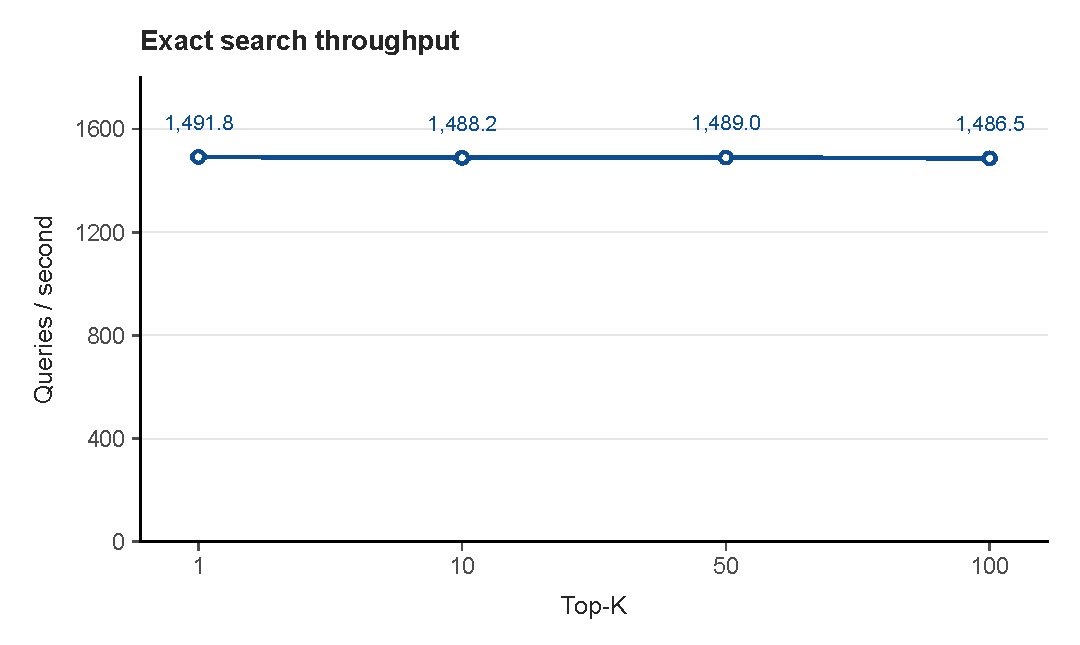
\includegraphics[width=0.90\linewidth,height=76mm,keepaspectratio]{figure-1.pdf}
\caption{精确检索吞吐与 K 的关系：标记为 3 次运行均值，误差条为样本标准差；小于标记尺度的误差条不易分辨}\label{fig:1}
\end{figure}

从 $K=1$ 增至 100，QPS 最大差异约为 0.36\%，P99 也基本保持不变。这与评分和完整基数排序均不依赖 $K$ 的结构一致，增加 $K$ 主要改变结果输出长度。结合第 7 节的内核时间分布，精确检索应优先改善评分阶段的并行映射和访存，再评估 Top-K 选择对整体性能的增益。


\begin{figure}[H]
\centering
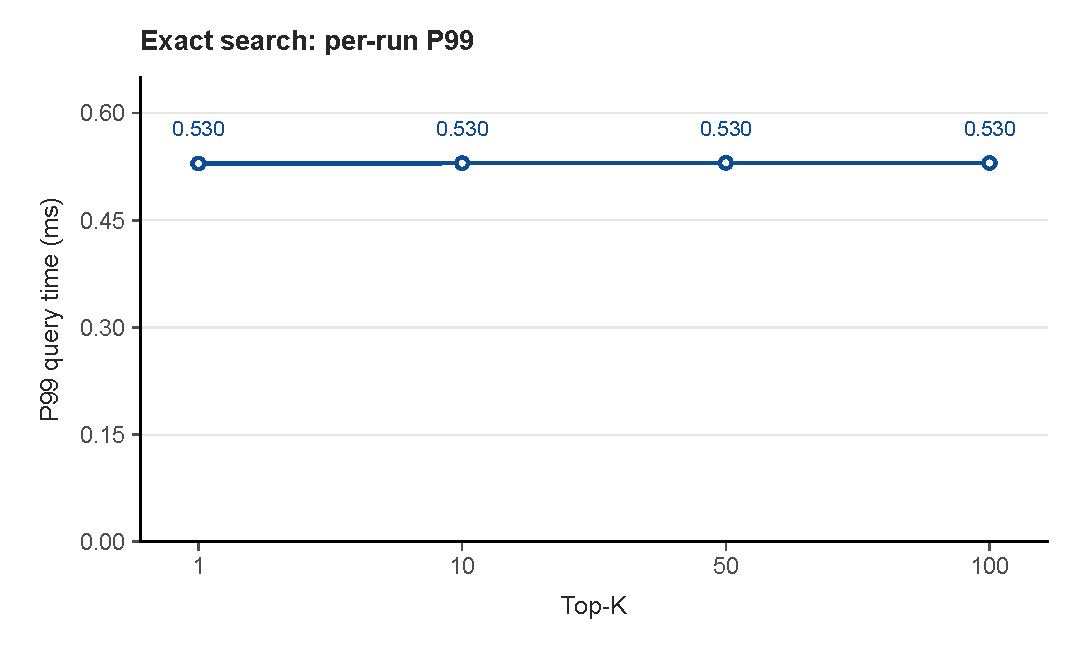
\includegraphics[width=0.90\linewidth,height=76mm,keepaspectratio]{figure-2.pdf}
\caption{精确检索逐查询 P99 与 K 的关系：标记与误差条为 3 个运行级 P99 的均值和样本标准差，不是单查询尾部置信区间}\label{fig:2}
\end{figure}

设备工作集估算为 548,183,295 bytes（约 522.8 MiB），主要由$10^6\times128$ 个 FP32 数据元素和排序工作区组成，在本次显存容量内有充分余量。


\subsection{IVF 探测桶数的权衡}

固定 $K=10$、批大小为 128，表 4 汇总不同探测桶数的结果，图 3-5 分别展示吞吐、P99 和召回率。所有召回率均以同一组 20 条 CPU 精确检索结果为真值。


\par\medskip\noindent\begin{minipage}{\linewidth}
\footnotesize
\captionof{table}{IVF-Flat 在不同探测桶数下的性能与质量}\label{tab:4}
\begin{tabular}{@{}C{13.520mm}R{14.232mm}R{28.464mm}R{15.655mm}R{15.655mm}R{19.925mm}R{17.790mm}R{17.078mm}@{}}
\toprule
\mbox{\textbf{探测桶数}} & \mbox{\textbf{Recall@10}} & \mbox{\textbf{QPS 均值\ensuremath{\pm}标准差}} & \mbox{\textbf{P50/ms}} & \mbox{\textbf{P99/ms}} & \mbox{\textbf{候选数/查询}} & \mbox{\textbf{采样加速比}} & \mbox{\textbf{工作集/MiB}} \\
\midrule
1 & 1.0 & $1327.588\pm3.136$ & 0.592813 & 0.634965 & 467.405 & $125.51\times$ & 488.417 \\
4 & 1.0 & $1086.391\pm2.829$ & 0.766684 & 0.883830 & 5934.018 & $95.20\times$ & 488.740 \\
16 & 1.0 & $633.063\pm0.680$ & 1.411880 & 1.671482 & 27008.017 & $53.57\times$ & 489.764 \\
64 & 1.0 & $246.517\pm0.099$ & 3.759094 & 4.307572 & 87433.332 & $19.11\times$ & 492.337 \\
256 & 1.0 & $97.927\pm1.488$ & 9.717852 & 11.390438 & 220088.434 & $7.70\times$ & 497.894 \\
\bottomrule
\end{tabular}
\end{minipage}\par\medskip

即使 $\mathrm{nprobe}=1$ 时平均仅评分 467.4 个候选，IVF 的 QPS 仍比 GPU精确检索低 10.8\%；$\mathrm{nprobe}=16$ 时低 57.5\%。候选缩减和较小的临时缓冲区尚未转化为完整查询加速。结合实现结构，CPU 粗检索、候选 ID 排序与传输是后续应分段测量的成本来源；现有结果支持进一步研究设备端粗检索与候选收集。


\begin{figure}[H]
\centering
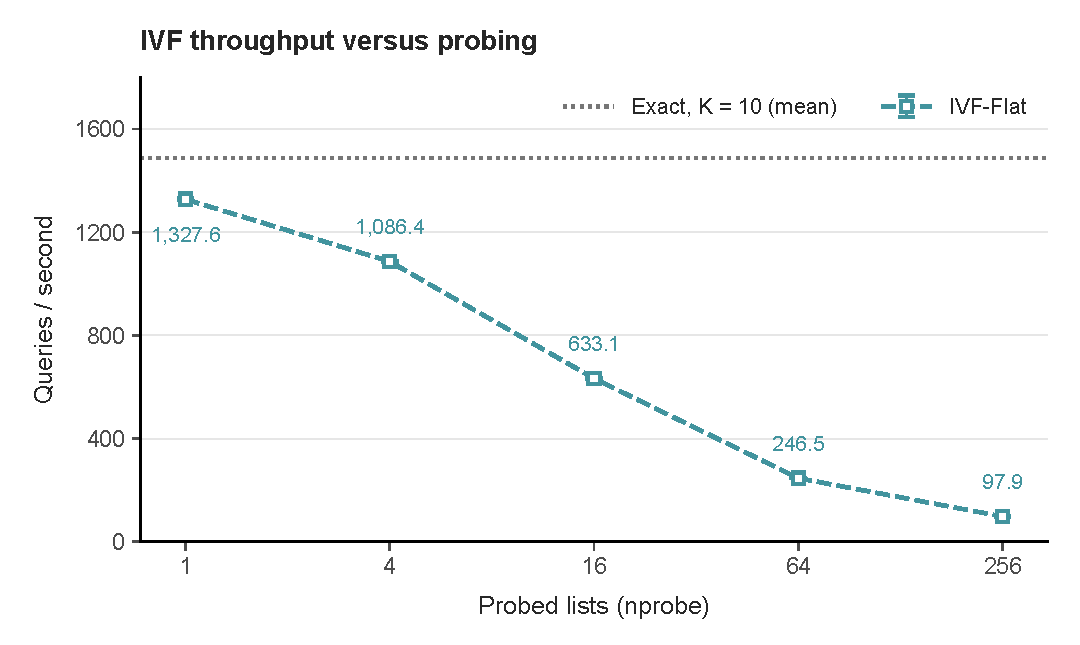
\includegraphics[width=0.90\linewidth,height=76mm,keepaspectratio]{figure-3.pdf}
\caption{IVF 吞吐与探测桶数的关系：5 次均值及样本标准差，K=10；灰色水平线为精确检索 K=10 的均值}\label{fig:3}
\end{figure}

\begin{figure}[H]
\centering
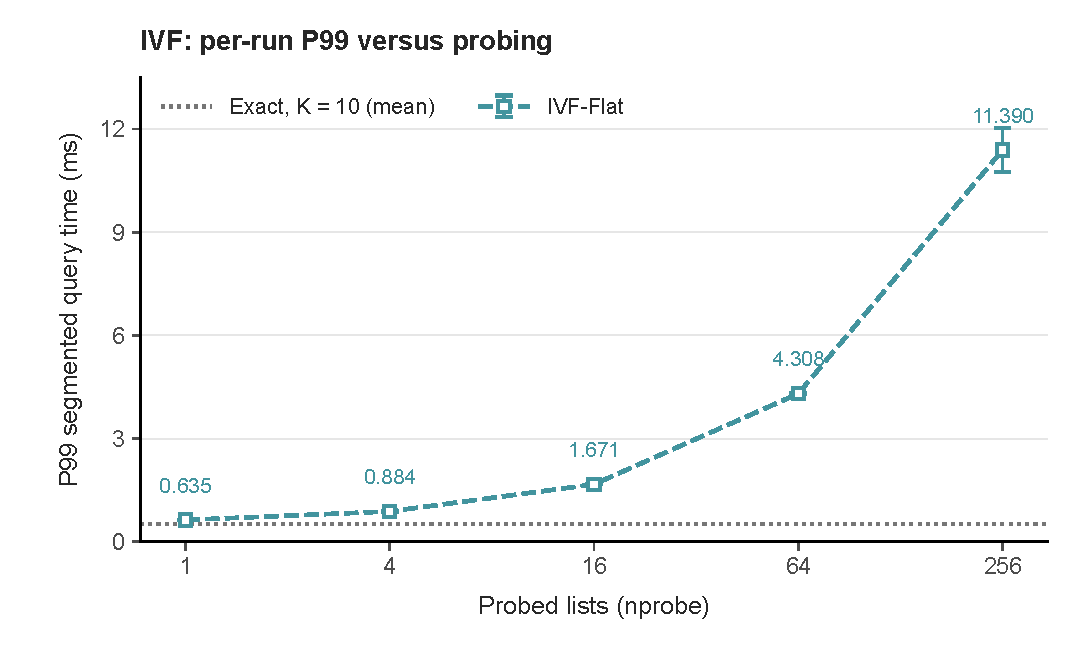
\includegraphics[width=0.90\linewidth,height=76mm,keepaspectratio]{figure-4.pdf}
\caption{IVF 分段查询计时 P99 与探测桶数的关系：5 个运行级 P99 的均值及样本标准差；灰色线为精确检索对照}\label{fig:4}
\end{figure}

探测桶数从 1 增至 256 时，平均候选数从约 467 增至 220,088，QPS 下降约92.6\%，P99 增至约 17.9 倍，而 Recall@10 保持为 1。


\begin{figure}[H]
\centering
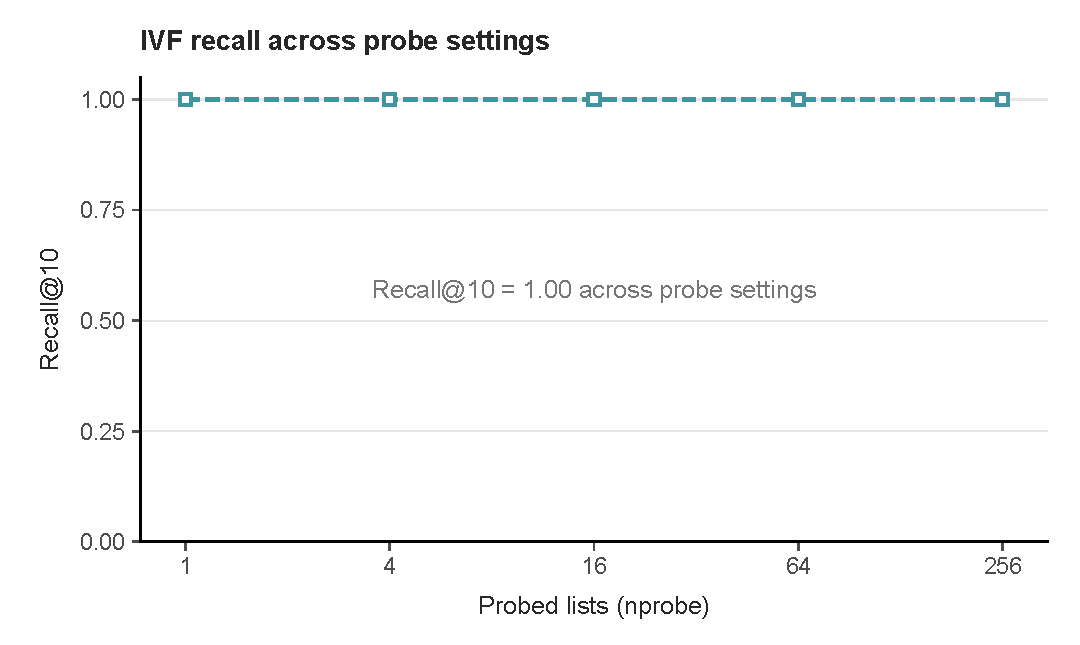
\includegraphics[width=0.90\linewidth,height=76mm,keepaspectratio]{figure-5.pdf}
\caption{IVF Recall@10 与探测桶数的关系（同一组 20 条质量查询）}\label{fig:5}
\end{figure}

五个工作点的平均位置分数误差均为 $1.28857791424\times10^{-7}$，与精确检索 $K=10$ 相同。因此，在本次易分簇数据和 20 条质量查询上，增加探测桶数只增加了成本，未带来可观察的召回收益。


\subsection{批大小敏感性}

固定 $K=10$、$\mathrm{nprobe}=16$，结果见表 5 和图 6-7。


\par\medskip\noindent\begin{minipage}{\linewidth}
\small
\captionof{table}{查询分组大小对 IVF-Flat 的影响}\label{tab:5}
\begin{tabular}{@{}C{24.657mm}R{24.657mm}R{24.657mm}R{24.657mm}R{24.657mm}R{24.657mm}@{}}
\toprule
\textbf{批大小} & \textbf{Recall@10} & \textbf{QPS 均值} & \textbf{QPS 标准差} & \textbf{P50/ms} & \textbf{P99/ms} \\
\midrule
1 & 1.0 & 630.618 & 6.547 & 1.416869 & 1.673444 \\
32 & 1.0 & 618.565 & 32.478 & 1.418684 & 1.674368 \\
128 & 1.0 & 631.302 & 2.933 & 1.411555 & 1.670336 \\
\bottomrule
\end{tabular}
\end{minipage}\par\medskip

\begin{figure}[H]
\centering
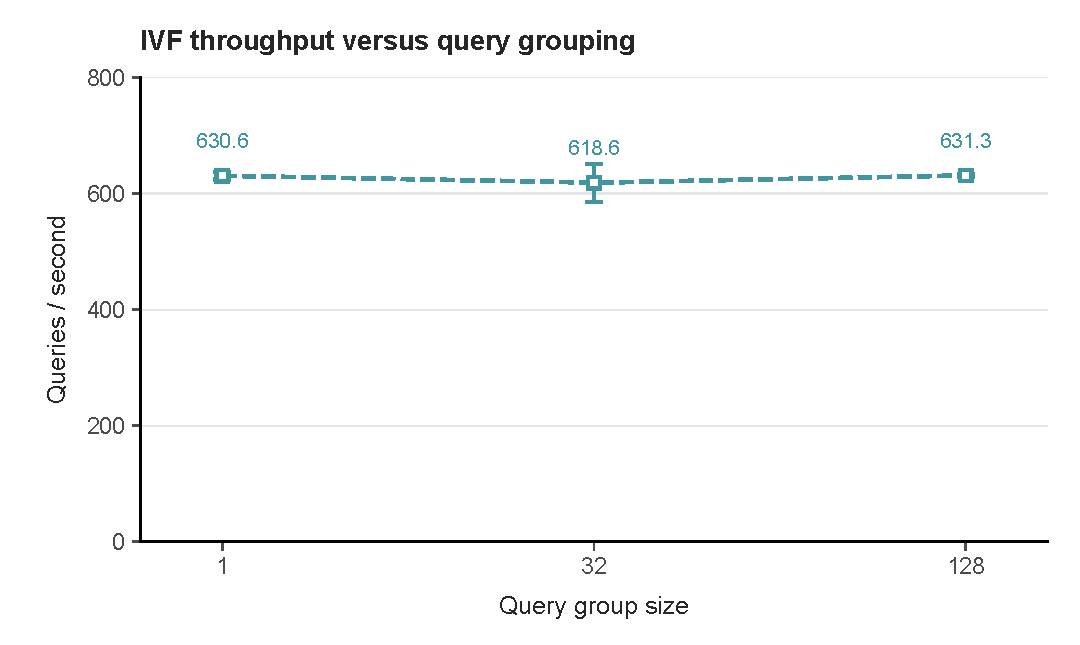
\includegraphics[width=0.90\linewidth,height=76mm,keepaspectratio]{figure-6.pdf}
\caption{IVF 吞吐与查询分组大小的关系：5 次运行均值及样本标准差；分组参数不代表多查询并发}\label{fig:6}
\end{figure}

批大小为 1 和 128 时，QPS 均值仅相差约 0.11\%；批大小为 32 时，样本标准差为 32.48 QPS，高于另两组。三个工作点未呈现随批大小增大而单调增加的吞吐，与当前逐查询同步执行的结构一致。


\begin{figure}[H]
\centering
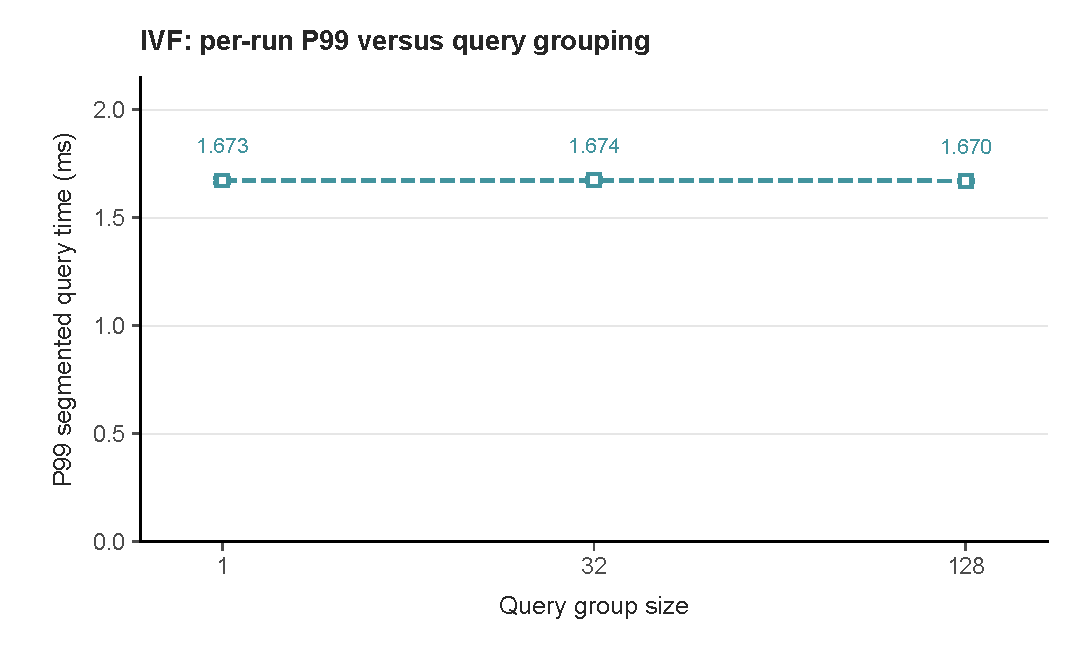
\includegraphics[width=0.90\linewidth,height=76mm,keepaspectratio]{figure-7.pdf}
\caption{IVF 分段查询计时 P99 与查询分组大小的关系：5 个运行级 P99 的均值及样本标准差}\label{fig:7}
\end{figure}

三组召回率均为 1，平均位置分数误差均为$1.28857791424\times10^{-7}$。本实验用于诊断当前分组接口，尚未涉及真正的多查询并行调度，也未进行组间显著性检验。


\section{性能剖析与瓶颈分析}

Nsight Systems 分别采集 $K=10$ 的精确检索和 $K=10$、$\mathrm{nprobe}=16$的 IVF 检索。两者使用相同百万级数据库、$Q=1000$ 和批大小 128，质量查询数降为 1，以减少事后 CPU 验证成本。GPU 内核、CUDA API 与 GPU 传输统计各自使用独立的时间分母；同步 API 的等待可能覆盖设备执行时间，因此本文分别解释三类统计。前节未插桩实验用于报告正式吞吐，本节采样用于定位成本 \cite{r10}。


\subsection{精确检索：评分占主导}

{\small\ttfamily score\_\allowbreak{}ca\allowbreak{}ndidates\allowbreak{}\_\allowbreak{}kernel} 的 1000 次执行合计 443.36 ms，占 GPU 内核时间的 89.5\%；CUB 基数排序内核合计约 52.17 ms，占 10.5\%。主机 API 统计中，{\small\ttfamily cudaMemcpy} 调用 3001 次，合计 512.17 ms（75.5\%）；{\small\ttfamily cudaMalloc} 调用 7 次，合计 131.40 ms（19.4\%）。设备 H2D 传输合计 27.62 ms，其中包含约 512 MB数据库的首次上传。


最大单次 H2D 为 27.342 ms，对应初始数据库上传；剩余 1000 次查询上传合计约 0.278 ms。API 中的高传输调用占比同时包含同步等待，设备实际传输与主机等待须分开解释。


采用 Amdahl 的部分改进分析 \cite{r11}，设某阶段占所考察时间的比例为 $f$，改进倍数为 $a$。其他阶段保持不变时，整体加速及其理想上界为


\nopagebreak[4]
\begin{equation}
\label{eq:8}
S(a)=\frac{1}{(1-f)+f/a},\qquad
\lim_{a\to\infty}S(a)=\frac{1}{1-f}.
\end{equation}

若理想地消除全部排序，精确检索内核部分的上限约为$1/(1-0.105)=1.12$ 倍，完整查询的改善还会更小。因此优先优化评分映射和访存更符合当前成本分布；长期服务接口还可跨调用复用数据库与工作区，摊薄冷启动开销。


\subsection{IVF：设备排序与主机处理成本}

IVF 评分内核的 1000 次执行合计 13.44 ms，占 GPU 内核时间的 32.9\%；CUB排序合计约 27.41 ms，占 67.1\%。候选缩减后，评分成本下降，完整排序成为设备端的主要开销。API 侧 {\small\ttfamily cudaMemcpy} 调用 4001 次，合计 235.00 ms（57.2\%）；{\small\ttfamily cudaMalloc} 调用 8 次，合计 140.48 ms（34.2\%）。H2D 设备传输合计 167.64 ms，其中初始数据库上传为 162.737 ms，余下 2000 次查询与候选上传合计约 4.902 ms。


图 8 对照两条路径的设备内核时间构成，展示评分与排序的相对占比变化。该比例以内核时间合计为分母，不包含 CPU 粗检索或初始化，因而用于确定设备端优化优先级，不替代完整查询时间比较。


\begin{figure}[H]
\centering
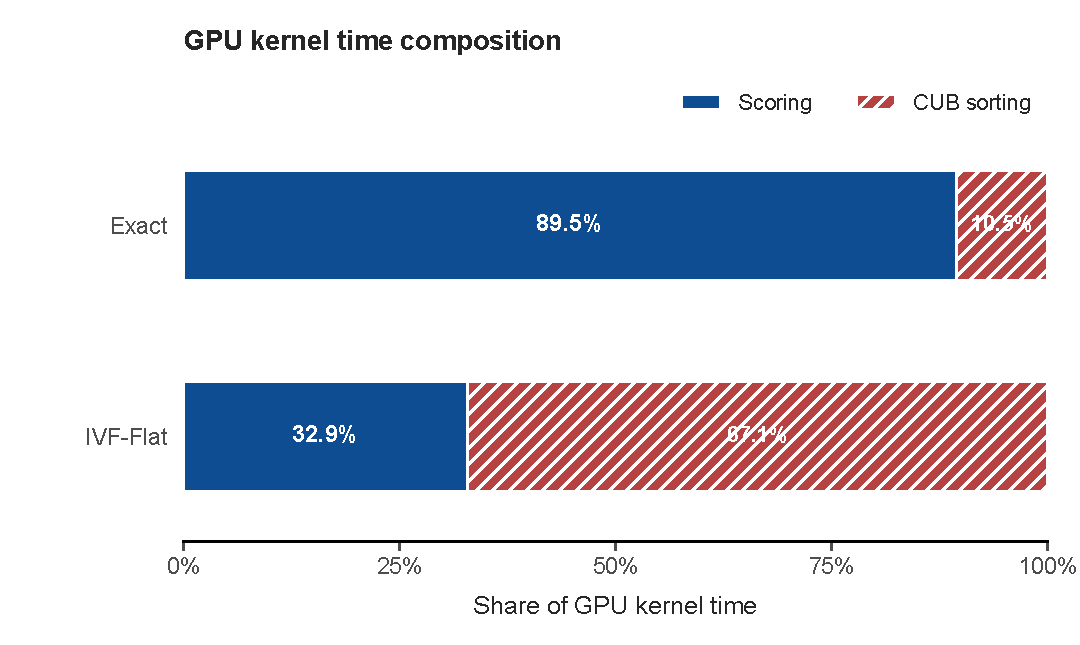
\includegraphics[width=0.90\linewidth,height=76mm,keepaspectratio]{figure-8.pdf}
\caption{精确检索与 IVF 的 GPU 内核时间构成：每条路径各一次 nsys 采样，以评分与 CUB 排序内核累计时间为分母；不含主机 API 和传输时间}\label{fig:8}
\end{figure}

初始上传在两次独立采样中波动较大，稳态比较应聚焦查询阶段。尽管评分内核已从精确检索的 443.36 ms 减少到 13.44 ms，IVF 的完整查询吞吐仍更低。该结果说明设备内核之外的成本决定了候选缩减能否转化为实际加速。后续可用 NVTX标记中心排序、ID 拼接与排序、索引加载和设备执行，进一步分解时间。


设备端可优先比较块内 Top-K 选择与层次归并。作为对照，若只消除评分内核，按其 32.9\% 占比计算的内核加速上限约为 $1/(1-0.329)=1.49$ 倍。因此，减少主机候选处理、构建设备常驻倒排结构并改善选择算法，比单独优化候选评分更值得优先验证。


\subsection{性能计数器的采集限制}

受宿主机性能计数器访问权限限制，两条检索路径均未获得 Nsight Compute测量结果 \cite{r12}。本次分析采用 Nsight Systems 的内核、API 与传输时间；DRAM/L2吞吐、占用率、寄存器使用及停顿原因尚无测量值。


\section{数值验证与实现讨论}

\subsection{数值判定与证据层次}

近同分候选的判定需要区分排序差异与检索错误。严格比较每个返回位置时，即使 ID集合完全一致、评分误差仅为 $10^{-7}$ 量级，位置交换仍会触发失败。本文验证同时保留严格排序与容差排序结果，并以完整 ID 集合相同和评分容差作为接受换位的条件，使数值舍入与真实检索错误可以分别观察。


性能评价同时考虑完整查询吞吐和分阶段成本。百万级输入上的参数扫描揭示候选规模、查询分组与吞吐之间的关系；Nsight Systems 则提供设备内核、主机API 和传输三个视角。结合两类测量，可判断候选缩减是否转化为实际收益，避免仅凭评分内核变快推断完整查询加速。


实现层面已采用调用内缓冲复用、GPU 聚类分配、CSR 倒排结构和确定性同分排序。单元测试覆盖三种度量、$K$ 范围、FP16 解码、零范数余弦、索引保存/加载、非法参数和损坏文件；Python 测试另行覆盖容差判定。当前结果评价这些设计组合后的表现，各项优化的独立贡献仍需逐项消融测量。


\subsection{可验证的优化假设}

第一项假设是精确评分受当前访存映射约束。可在同一数据库和评分精度下，比较一线程一向量与一线程束一向量，保持 Top-K 阶段不变，同时记录评分内核时间、完整调用 QPS 和结果误差。若评分缩短而完整吞吐变化很小，说明其他阶段限制了收益；若评分未改善，则应进一步检查归约代价和寄存器压力。取得计数器权限后，再利用内存事务与吞吐验证原因。CUDA 合并访存原则为这一假设提供设计依据 \cite{r9}，目前的 nsys 时间占比本身不能证明带宽已经饱和。


第二项假设是 IVF 的主机粗检索与候选处理抵消了部分设备收益。验证时应先为索引加载、中心评分、ID 拼接、ID 排序和设备执行分别加入时间标记，再逐项替换为设备端实现。对照中固定中心和候选集合，可以将执行位置变化与近似质量变化分开；若完整调用时间下降但候选数或召回率也改变，则需另行解释算法差异。进一步的常驻索引实验应把首次上传与连续请求分开计时，从而判断收益来自数据驻留还是候选生成本身。


第三项假设涉及选择算法。RadiK 将基数选择阈值与结果筛选分开，说明返回Top-K 集合并不必然要求全量排序 \cite{r6}。但本任务要求有序结果，并采用同分 ID规则，因此替换 CUB 时还需计入最终 $K$ 个元素排序与边界同分处理。可在固定候选分数数组上比较全排序、块内选择加归并和基数选择，同时覆盖随机分数、大量重复值与集中分布。只有在相同输出约束下仍降低时间，才构成有效的选择阶段改进；其完整查询收益还受第 7 节成本占比约束。


批量并行则应作为独立实验维度：先固定每个查询的候选和评分，再改变同时驻留的查询数，测量吞吐、工作集与逐请求完成时间。实际多查询并发会改变资源竞争和排队情况，不能由当前分组参数的扫描外推。上述实验分别检验评分映射、主机分工和选择策略，使优化结论能够对应到具体机制。


\section{有效性威胁、局限与后续工作}

首先，合成查询由库向量扰动产生，数据容易分簇；20 条质量查询也不足以代表真实嵌入数据的难度分布。因此，所有探测桶数均取得满召回，是本次输入和样本上的观察。重复运行相同查询只增加时间测量次数，不扩大质量样本。正式性能还限于单卡 RTX 5090、L2 度量和 $\mathrm{nlist}=4096$；内积聚类的设计尚需在独立数据上评估。


其次，CPU 加速比基于单线程参考实现的 20 条采样查询，尚无多核优化或 FAISS对照；环境归档也缺少 CPU 精确型号、线程亲和和频率控制记录。设备工作集是显式分配合计，不包含上下文与驱动开销，整进程显存峰值尚未采集。IVF 单查询计时按分段相加，服务排队与在线响应延迟不在本实验范围内。


最后，FP16 仅作为文件输入格式，当前验证针对解码后相同输入的 CPU/GPU一致性，没有评估相对原始 FP32 数据的量化损失，也没有原生低精度计算收益。独立 CPU/GPU 聚类一致性、各项优化消融和硬件计数器分析仍待补充。


据现有证据，后续工作可按以下顺序开展：


\par\noindent\hangindent=1.2em\hangafter=1\textbullet\quad 对精确检索比较线程束协同评分与分块布局，再评估块内 Top-K 和层次归并，同时报告内核与完整查询收益。\par

\par\noindent\hangindent=1.2em\hangafter=1\textbullet\quad 将 IVF 粗检索与候选收集迁移到 GPU，延长数据库、倒排表和工作区的驻留周期；配合多查询评分与分段选择，形成真正的批量并行执行。\par

\par\noindent\hangindent=1.2em\hangafter=1\textbullet\quad 在公开嵌入数据集上扩大质量查询数与种子数量，加入 FAISS {\small\ttfamily IndexFlat} 和{\small\ttfamily IndexIVFFlat} 同口径对照，建立有区分度的召回率-延迟曲线。\par

\par\noindent\hangindent=1.2em\hangafter=1\textbullet\quad 在取得计数器权限后验证访存、占用率与停顿假设；随后探索 FP16/BF16 设备存储和计算，综合评估显存、吞吐及召回率。\par

\section{结论}

本文实现了 GPU 精确检索与可持久化 IVF-Flat 索引，在 $N=10^6$、$D=128$、$Q=1000$ 的规模上完成验证与性能评估。精确检索在 $K=1$ 至 100 时保持约1.49k QPS；IVF 在 $\mathrm{nprobe}=1$ 时对 20 条质量查询取得满召回，但1327.6 QPS 仍低于精确检索。候选缩减虽降低设备评分成本，其收益受到完整查询流程中其他开销的制约。


性能剖析进一步区分了精确检索的评分热点与 IVF 的排序热点，批大小扫描则反映当前串行调度的局限。由此得到的优化方向是改进评分映射、迁移粗检索与候选处理、优化 Top-K 选择，并建立真正的批量并行执行。本文提供了对应的源码、测试、固定配置和可复算结果，为这些后续改进建立了明确基线。这些结论适用于本次合成数据、单卡和同步执行方式；现有证据支持对实现成本的分析，而非对不同近邻算法作普遍排名。进一步扩大独立质量查询集并加入同口径成熟库对照，才能评价该实现对实际嵌入检索工作负载的适用程度。


\appendix

\section{复现方法}

源代码包含数据生成、索引构建、检索及验证脚本。逐次与汇总结果保存在{\small\ttfamily report\_\allowbreak{}a\allowbreak{}ssets/\allowbreak{}ev\allowbreak{}idence/\allowbreak{}}；百万级输入和索引按第2节参数重新生成。


\needspace{12\baselineskip}

在 Linux/CUDA 主机从 {\small\ttfamily task-\allowbreak{}09-\allowbreak{}gpu-\allowbreak{}vect\allowbreak{}or-\allowbreak{}searc\allowbreak{}h/\allowbreak{}} 执行。以下架构参数 120 对应本次 RTX 5090；其他 GPU 须使用对应架构。本地 CPU 回归可使用{\small\ttfamily -\allowbreak{}DENABLE\allowbreak{}\_\allowbreak{}CUDA=OF\allowbreak{}F} 构建。


\par\needspace{9\baselineskip}
\begin{ReportCode}
cmake -S . -B build-cuda128-root \
  -DCMAKE_BUILD_TYPE=Release -DENABLE_CUDA=ON \
  -DCMAKE_CUDA_ARCHITECTURES=120 \
  -DCMAKE_CUDA_COMPILER=/usr/local/cuda-12.8/bin/nvcc \
  -DCMAKE_CUDA_FLAGS=-lineinfo
cmake --build build-cuda128-root --parallel
ctest --test-dir build-cuda128-root --output-on-failure
\end{ReportCode}

\needspace{9\baselineskip}

依照 README 安装 Python 依赖后，使用新的输出目录运行完整实验：


\par\needspace{6\baselineskip}
\begin{ReportCode}
python3 scripts/run_task9_experiments.py \
  --binary build-cuda128-root/vector_search \
  --output-dir outputs/task9_report_reproduction \
  --preset report
\end{ReportCode}

性能剖析可在允许权限的机器追加 {\small\ttfamily -\allowbreak{}-\allowbreak{}profil\allowbreak{}e-\allowbreak{}tools \allowbreak{}ncu nsys\allowbreak{}}，或使用{\small\ttfamily scripts/\allowbreak{}profile\_\allowbreak{}vector\_\allowbreak{}s\allowbreak{}earch.\allowbreak{}py\allowbreak{}} 补采；中断后保持输入参数不变，并使用{\small\ttfamily -\allowbreak{}-\allowbreak{}resume}。


\needspace{12\baselineskip}\begingroup\small\linespread{1.0}\selectfont\begin{thebibliography}{99}\setlength{\itemsep}{1pt}\setlength{\parskip}{0pt}

\bibitem{r1}Johnson, J., Douze, M., and Jégou, H. \emph{Billion-scale similarity search with GPUs}. arXiv:1702.08734, 2017. \href{https://arxiv.org/abs/1702.08734}{论文原文}。

\bibitem{r2}Douze, M., Guzhva, A., Deng, C., Johnson, J., Szilvasy, G., Mazaré, P.-E., Lomeli, M., Hosseini, L., and Jégou, H. (2024). \emph{The Faiss Library}. arXiv:2401.08281v1. \href{https://arxiv.org/abs/2401.08281v1}{论文原文}。

\bibitem{r3}Jégou, H., Douze, M., and Schmid, C. (2011). Product Quantization for Nearest Neighbor Search. \emph{IEEE Transactions on Pattern Analysis and Machine Intelligence}, 33(1), 117-128. \href{https://doi.org/10.1109/TPAMI.2010.57}{DOI}。

\bibitem{r4}Malkov, Y. A. and Yashunin, D. A. (2018). \emph{Efficient and Robust Approximate Nearest Neighbor Search Using Hierarchical Navigable Small World Graphs}. arXiv:1603.09320v4. \href{https://arxiv.org/abs/1603.09320v4}{作者预印本}。

\bibitem{r5}Aumüller, M., Bernhardsson, E., and Faithfull, A. (2020). ANN-Benchmarks: A Benchmarking Tool for Approximate Nearest Neighbor Algorithms. \emph{Information Systems}, 87, 101374. \href{https://doi.org/10.1016/j.is.2019.02.006}{DOI}。

\bibitem{r6}Li, Y., Zhou, B., Zhang, J., Wei, X., Li, Y., and Chen, Y. (2024). RadiK: Scalable and Optimized GPU-Parallel Radix Top-K Selection. \emph{Proceedings of the 38th ACM International Conference on Supercomputing}, 537-548. \href{https://doi.org/10.1145/3650200.3656596}{DOI}，\href{https://arxiv.org/abs/2501.14336}{作者预印本}。

\bibitem{r7}NVIDIA. \emph{CUB DeviceRadixSort: Stable Device-Wide Radix Sorting}. \href{https://github.com/NVIDIA/cccl/blob/main/cub/cub/device/device_radix_sort.cuh}{官方实现与说明}。

\bibitem{r8}Lloyd, S. P. (1982). Least Squares Quantization in PCM. \emph{IEEE Transactions on Information Theory}, 28(2), 129-137. \href{https://doi.org/10.1109/TIT.1982.1056489}{DOI}。

\bibitem{r9}NVIDIA. \emph{CUDA C++ Best Practices Guide, CUDA Toolkit 12.8}. \href{https://docs.nvidia.com/cuda/archive/12.8.0/cuda-c-best-practices-guide/}{官方文档}。

\bibitem{r10}NVIDIA. \emph{Nsight Systems User Guide}. \href{https://docs.nvidia.com/nsight-systems/UserGuide/index.html}{官方文档}。

\bibitem{r11}Amdahl, G. M. (1967). Validity of the Single Processor Approach to Achieving Large Scale Computing Capabilities. \emph{Proceedings of the AFIPS Spring Joint Computer Conference}, 483-485. \href{https://doi.org/10.1145/1465482.1465560}{DOI}。

\bibitem{r12}NVIDIA. \emph{ERR\_NVGPUCTRPERM: Permission Issue with Performance Counters}. \href{https://developer.nvidia.com/ERR_NVGPUCTRPERM}{官方说明}。

\end{thebibliography}\endgroup
\end{document}
